\documentclass[a4paper]{article}

%% Language and font encodings
\usepackage[english]{babel}
\usepackage[utf8x]{inputenc}
\usepackage[T1]{fontenc}

%% Sets page size and margins
\usepackage[a4paper,top=3cm,bottom=2cm,left=3cm,right=3cm,marginparwidth=1.75cm]{geometry}

%% Useful packages
\usepackage{amsmath}
\usepackage{float}
\usepackage{graphicx}
\usepackage[colorinlistoftodos]{todonotes}
\usepackage[colorlinks=true, allcolors=blue]{hyperref}
\usepackage{minted}
\usepackage{lmodern}

\usepackage{tikz}
\usetikzlibrary{arrows,positioning,fit,shapes,calc}
\usepackage{algorithm}
\usepackage[noend]{algpseudocode}

\title{Distributed systems}
\author{Oechsel Pierre}


\tikzset{
  treenode/.style = {align=center, inner sep=0pt, text centered, font=\sffamily},
  slave/.style = {treenode, circle, draw, text width=1.5em},
  master/.style = {treenode, circle, draw=red, text width=8em},
}

\begin{document}

\maketitle

\section{First steps}

The main goal of my project was to build a \textbf{decentralized and fault tolerant} network.
Before implementing my current solutions, I thought during a few weeks about other approaches. Even though I didn't implemented them I will write a bit about them.

\subsection{Back to centralisation}

My first thought on which topology to choose was to select the tree topology. Under the condition that the tree is balanced broadcasting, scattering and electing a leader can be done efficiently \cite{tel2000introduction}. We suppose the existence of a master node, which we call \textit{oracle} which maintains a coherent view of the topology. He acts as a server and allows us to maintain the topology of a balanced tree. Adding new node to this tree is not difficult. If one node of the tree fails and become dead, this oracle allows us to rebuild the topology \cite{huang2005performance}. Nodes of the distributed systems are only keeping few informations about the topology: their father and their childs. The root of the tree is linked to the \textit{oracle}.

But the \textit{oracle} can also fail. This event is dramatic: without the oracle we can't maintain a coherent topology anymore. If the root of tree then fails our tree will be splitted in two components without any hopes to restore the situation.
In order to fix this problem, we do not have one \textit{oracle}, but several. They are all linked to each other (here in red). Each oracles are keeping the same copy of the topology.
Now, adding(and updating after a node has failed) a new node to the topology is a bit more tricky. Each node now have two status: either it is an \textit{oracle}, either it is a normal node. So when we are performing operations in order to maintain the topology (like adding a node), a node can switch from being a "basic node" to an "oracle". But under which conditions do we want to execute this switch? This question is tricky as we want to maintain what is stored in the distributed system. The priority should be to always have at least two oracles, but sometimes we might consider it interesting to have more basic nodes.

The previous difficulty and the fact that this idea required to create two different distributed systems (one fully connected for the \textit{oracle} and one in tree topology for the other nodes) prevented me from implementing it.



\begin{figure}[H]
    \centering
    \begin{tikzpicture}[-,level/.style={sibling distance = 8cm/#1,level distance = 1.5cm}, level 1/.style={level distance=2cm}] 
\node [master] {}
    child{node [slave] {}
    child{node [slave] {} 
            child{node [slave] {} 
            	child{node [slave] {} }
							child{node [slave] {}}
            }
            child{node [slave] {}
							child{node [slave] {}}
							child{node [slave] {}}
            }                            
    }
    child{node [slave] {}
            child{node [slave] {} 
            }
            child{node [slave] {}
            }
    }}
; 



\draw (0*360/3: 1cm) node[slave] (sA) {};
\draw (1*360/3: 1cm) node[slave] (sB) {};
\draw (2*360/3: 1cm) node[slave] (sC) {};
 
 \draw[-] (sA) -- (sB);
 \draw[-] (sA) -- (sC);
 \draw[-] (sB) -- (sC);
\end{tikzpicture}
\caption{Three master nodes and  12 basic nodes}
\end{figure}


\subsection{Second idea, ring topology}

Even though the ring topology appear useless because it's not very performant on paper (if we have $n$ nodes and the links are bi-directionnal, we need at least $\frac{n}{2}$ messages for a broadcast for example), its simplicity makes it very interesting for this assignement. So I began to investigate ways to keep this simplicity while allowing it to scale a bit more.
In the end, I had the following idea:
We keep the ring topology. However the nodes of this topology are no more a single agent, but are clusters of $m$ agents.
Inside a cluster all the agents are connected using a fully connected topology. This allow for high performance and also efficiency against failure.

The biggest trick comes from how we are connecting one cluster with the following cluster. We might be tempted by the idea that in each cluster their exists one node that is pointing toward the a node of the next cluster. However, this is a bad idea as we have a point of failure between clusters. We want to avoid this: if a cluster is disconnected from the ring because this node failed we won't be able to reconnect it. My solution was to say the following, given a cluster $X = (x_1, \cdots x_m)$ and $Y = (y_1, \cdots y_m)$ that must be linked in the ring:
\begin{itemize}
    \item Select $\phi: [1, \cdots, m] \mapsto [1, \cdots, m]$ a bijective function.
    \item $x_1$ points toward $y_{\phi(1)}$
    \item $\cdots$
    \item $x_m$ points toward $y_{\phi(m)}$
\end{itemize}

So, even if a node of the cluster $Y$ fails, $X$ is not disconnected as it possess an agent connected to another agent of $Y$.

One other advantage of this approach is that we can adapt existing algorithms for broadcasting, scattering and leader election by combining an algorithm efficient for a ring topology and an algorithm efficient for a fully connected topology.

Unfortunately, as the protocols for adding a new node, or maintaining a topology after a node fails, seemed too long to create and test in the time I had I chose not to go further with this idea.


\begin{figure}[H]
    \centering
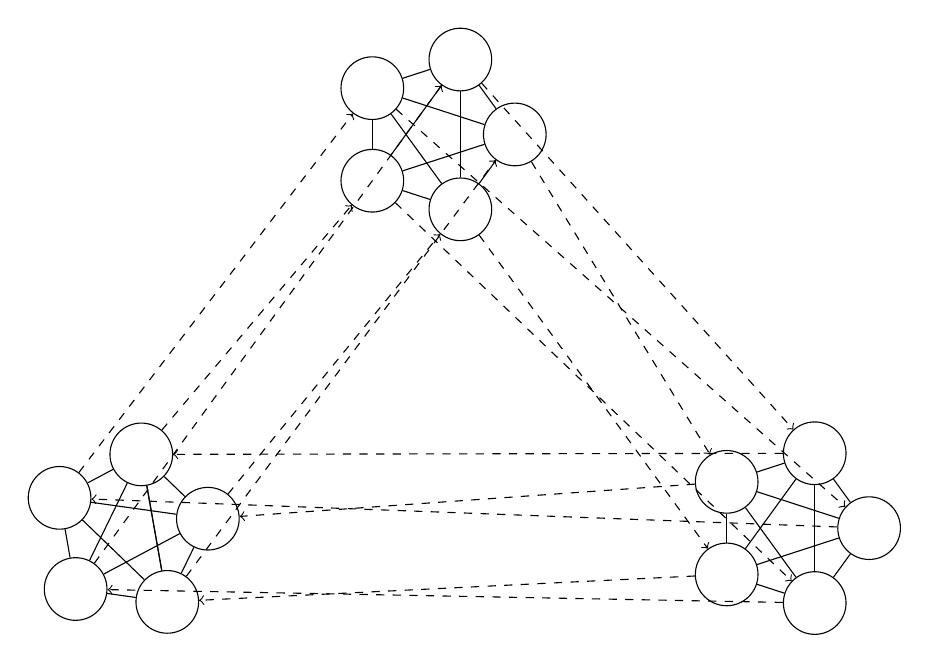
\begin{tikzpicture}[-,level/.style={sibling distance = 5cm/#1,level distance = 1.5cm}] 
\begin{scope}[local bounding box=scope1]
\draw (0*360/5+10: 1cm) node[circle, draw=black, text width=1.5em] (sA) {};
\draw (1*360/5+10: 1cm) node[circle, draw=black, text width=1.5em] (sB) {};
\draw (2*360/5+10: 1cm) node[circle, draw=black, text width=1.5em] (sC) {};
\draw (3*360/5+10: 1cm) node[circle, draw=black, text width=1.5em] (sD) {};
\draw (4*360/5+10: 1cm) node[circle, draw=black, text width=1.5em] (sE) {};
\end{scope}
\begin{scope}[shift={($(scope1.east)+(7cm,0)$)}]
\draw (0*360/5: 1cm) node[circle, draw=black, text width=1.5em] (bA) {};
\draw (1*360/5: 1cm) node[circle, draw=black, text width=1.5em] (bB) {};
\draw (2*360/5: 1cm) node[circle, draw=black, text width=1.5em] (bC) {};
\draw (3*360/5: 1cm) node[circle, draw=black, text width=1.5em] (bD) {};
\draw (4*360/5: 1cm) node[circle, draw=black, text width=1.5em] (bE) {};
\end{scope}
\begin{scope}[shift={($(scope1.east)+(2.5cm,5cm)$)}]
\draw (0*360/5: 1cm) node[circle, draw=black, text width=1.5em] (cA) {};
\draw (1*360/5: 1cm) node[circle, draw=black, text width=1.5em] (cB) {};
\draw (2*360/5: 1cm) node[circle, draw=black, text width=1.5em] (cC) {};
\draw (3*360/5: 1cm) node[circle, draw=black, text width=1.5em] (cD) {};
\draw (4*360/5: 1cm) node[circle, draw=black, text width=1.5em] (cE) {};
\end{scope}
 
\draw[-] (sA) -- (sB);
\draw[-] (sA) -- (sC);
\draw[-] (sA) -- (sD);
\draw[-] (sA) -- (sE);
\draw[-] (sB) -- (sC);
\draw[-] (sB) -- (sD);
\draw[-] (sB) -- (sE);
\draw[-] (sB) -- (sE);
\draw[-] (sC) -- (sD);
\draw[-] (sC) -- (sE);
\draw[-] (sD) -- (sE);



\draw[-] (bA) -- (bB);
\draw[-] (bA) -- (bC);
\draw[-] (bA) -- (bD);
\draw[-] (bA) -- (bE);
\draw[-] (bB) -- (bC);
\draw[-] (bB) -- (bD);
\draw[-] (bB) -- (bE);
\draw[-] (bB) -- (bE);
\draw[-] (bC) -- (bD);
\draw[-] (bC) -- (bE);
\draw[-] (bD) -- (bE);


\draw[-] (cA) -- (cB);
\draw[-] (cA) -- (cC);
\draw[-] (cA) -- (cD);
\draw[-] (cA) -- (cE);
\draw[-] (cB) -- (cC);
\draw[-] (cB) -- (cD);
\draw[-] (cB) -- (cE);
\draw[-] (cB) -- (cE);
\draw[-] (cC) -- (cD);
\draw[-] (cC) -- (cE);
\draw[-] (cD) -- (cE);


\path[->, dashed]
(sC) edge node {} (cC)
(sA) edge node {} (cE)
(sD) edge node {} (cB)
(sE) edge node {} (cA)
(sB) edge node {} (cD)

(bA) edge node {} (sC)
(bB) edge node {} (sB)
(bC) edge node {} (sA)
(bD) edge node {} (sE)
(bE) edge node {} (sD)

(cA) edge node {} (bC)
(cE) edge node {} (bD)
(cC) edge node {} (bA)
(cD) edge node {} (bE)
(cB) edge node {} (bB);

\end{tikzpicture}
\caption{Exemple for a ring of 3 clusters of 5 nodes}
\end{figure}


\section{Welcome Kademlia}

Finally after discussing with other people and doing a bit more of research I chose to implement something approaching Kademlia \cite{maymounkov2002kademlia}. This decision was supported by several reasons:
\begin{itemize}
    \item It allowed me to understand how a "real life" system was working
    \item Its simplicity was intriguing me
\end{itemize}

\subsection{Short description of Kademlia}

I strongly encourage you to read the original paper which is very well written. I'll write below a small overview of Kademlia, which given the hour at which I'm writting this part might be fuzzy and inexact.

Kademlia is focused around the \textit{xor distance}. Each node in the topology is associated to a unique 160-bits integer, called its id (here this integer is determined using a sha function). Two nodes of id $a$ and $b$ have a distance equal to $a \text{ xor } b$. This xor distance allows us to create easily a tree topology.
A Kademlia network is also associated to two parameters:
\begin{itemize}
    \item $K$: this is a number inversely proportional to the number of crashes we can expect in one hour. Here it is set to $20$.
    \item $\alpha$: the degree of parallelism for asynchronous communications, meaning we can have at most $\alpha$ communications at the same time.
\end{itemize}

One other key point is that to each node is associated a routing table. The routing table is divided in $160$ buckets. The bucket $i$ can contain at most $K$ nodes having an id $a$ with a xor distance to the current node (of id $id$) in the range $[2^{i-1}; 2^{i}]$ (so $a \text{ xor } b \in [2^{i-1}; 2^{i}]$). We say that our current node knows of an other node if this other node is present inside its routing table. Beware, the relation is not symmetric! When a node $a$ makes a communication with an other node $b$ (a ping, a node lookup / value lookup...), we try to had $a$ to the routing table of $b$. A node is added to the routing table if either a slot is disponible in the bucket or we can eject a non responsive node from this bucket. 

Kademlia is defined around three basic operations:
\begin{itemize}
    \item Ping: a node $a$ can ping a node $b$ in order to try to add $b$ to its routing table or to know if $b$ is alive
    \item Node find: a node $a$ can try to find the $K$ nearest node from a hash $h$ by iterating from node to node. The process to find the $K$ nearest node is done iteratively: First take, the $\alpha$ nearest node in our routing table. Then, for each entry of this list, ask the corresponding node for its $K$ nearest node in its routing table, merge it with our current list and keep the nearest $K$  node. We obtain a list of node $l'$. For each node in $l'$ we haven't already seen, get the $K$ nearest node in its routing table, merge and crop. Repeat until a fixpoint is achieve.
    \item value find: this is the same as a node find but we stop the exploration when a node contain a value.
\end{itemize}

From this basic operations, we can define more complex operations:
\begin{itemize}
    \item Storing a value: To store a value $v$, first compute the hash $h$ of $v$. Then, use a node find to get the $K$ nodes whose id are the nearest to $h$. Store $v$ in these $K$ nodes
    \item Retrieving a value: Use a value find operation (which is just an optimized node find as we stop the exploration as soon as we can)
    \item Connecting to an other node. A node $a$ can connect to a node $b$ by first pinging $b$, then asking for a node find of $id_a$.
\end{itemize}


We also have two other mechanism of refreshments. Firstly, every hour we take one representant per non updated in the last hours buckets and send a node find to them. This allow us to keep a up to date routing table aware of the newest change of topology. 
Secondly, we also refreshes stored values every hours by "republishing" them to the $K$ nearest nodes. This allows us to compensate for the connection and crash of nodes.


Finally, Kademlia is building a sort of tree topology with its routing table. The topology is always updating with each communications. Theorical performances is expected to be in the order of $O(log n)$ communications. We can also note that if we have few nodes (less than $160*k$, we can have a fully connected topology: every bucket could be filled, thus the routing table could contain $k*160$ nodes.

\subsection{Description of the questions done and approaches}

\subsubsection{Part 1}

\paragraph{Question 1:} Every questions was treated. However, for question 1)e we have a small nuance. Kademlia doesn't detect when a node crash. This could be done easily with monitors in erlang, but kademlia doesn't need to know that a node is dying: the routing table will be filled with connections to other nodes thanks to anterior communications and the mechanisms of republishing.

\paragraph{Question 2:} 
Broadcasting, scattering and leader election are quite absurd in kademlia. The goal of kademlia is to be able to scale, thus to avoir operations involving every nodes. Every operations aims to involve as few nodes as it can. Nevertheless, I've implemented a broadcast algorithm following \cite{czirkos2013solution}. I didn't really understood what was supposed to do scattering. Therefore, I've implemented it as a broadcast of every messages. Each node will be attributed a message taken uniformly randomly along the message lists: sharing informations on who picked which message would be too costly. We can hope that the messages are uniformly distributed among the nodes.

I haven't implemented a leader election algorithm. I tried, but as each node has a different view of the topology, and as a node $a$ can "know" of a node $b$ but the node $b$ can not know about the node $a$, the task isn't easy. My main lead was to adapt an algorithm of leader election for directed graphs described in \cite{tel2000introduction} (for exemple the one allowing us to convert a traversal algorithm to a leader election algorithm). However, the task was too complex for the time I had.


\subsubsection{Part 2}

UUID are computed as a 160-bit hash with sha. For now, we can only stored string, but I'm describing below a hypothetical way to share files. Sha1 algorithm aims to implement a hash function from cryptographic algorithm. Thus, we can hope that every hash can appear uniformly (ie for two values $a$ and $b$, we can't distinguish them from their hash values).

Every value is duplicated on $K$ nodes.

Question c) is not deterministic. If we are shutting down too much nodes at once, then the mechanism of key republishing could be too slow to happen. A solution will be to increase $K$. In normal use, no problem should occur with $K=20$ (see the original paper for more informations).

Question d) wasn't so easy. It is easy to release a data using a broadcast, but I didn't wanted to use it as it is against the "spirit" of Kademlia. An other idea would be to find the $K$ nearest nodes to the value and to delete the value from them. However, if a node near the value connected, this would not work as expected. Thus, I chose to remove the value from the $4K$ nearest nodes to it, and then to repeat the mechanism of removal 1 hour and 1 hour and a half after. In this time window value republishing is likely to have happened.

Question e) comes from properties of hash function (non distinguishability). In other words, if we expect the hash function to be "good", each node have the same chance to store a key. Thus, keys should be uniformly spread.

Question f) is directly in Kademlia. We are publishing values only on $K$ nodes. If new nodes connects, we could temporarly have more than $K$ nodes with the same key. However, the mechanism of key republishing will automatically remove the keys from nodes that became "far" regularly, which avoid us to flood the network.

\subsection{Part 3}

Nothing special to be said here, everything was done.





\section{Choice of implementations}

\subsection{OTP}

As I wanted to learn about erlang during this homework, I chose to follow OTP's guideline. This choice allowed me to have a code a bit cleaner, and mostly to use the full power of Erlang (supervisors, monitors, ...) in a simple way.
However, this decision drasticly decreases my development speed in a first time. As I wasn't a proficient erlang programmer at the start of the project, I spend a lot of time to understand simple things.

OTP also brought a big technical difficulty. Question 4.a asked to be able to spawn an agent remotely given a node name. Without OTP we only need to send the modules used by the agent to the remote node. Here, as I have an OTP application it is not as easy. Therefore, I've proceeded as follow:
\begin{itemize}
    \item Create a new module, \verb|client.erl| which contains everything needed to interact with other agents from the CLI. It is also responsible to start an agent on a remote node
    \item Send \verb|client.erl| to the remote node
    \item Zip the \verb|ebin| folder of the application
    \item Send it on the remote node
    \item Unzip it
    \item Add the destination folder on the remote node to its path
    \item Start the application on the remote note
\end{itemize}

\subsection{Asynchronicity}

Kademlia needs asynchronicity in order to work well. In the original paper, the author advises the use of UDP sockets. Instead, I chose to base myself upon erlang's communications. I still took great care to provide asynchrone method when I can. 
In order to ease my task, I took the following design decisions:
\begin{itemize}
    \item The routing table is executed by a gen\_server launched in another process. As such it is able to maintain a coherent state and to interact with the main process with messages
    \item Algorithms that can take a long time (node lookups, value lookups) are implemented as function executed in another process. For these algorithms I'm making sure to send $\alpha$ messages at the same time (at most).
    \item I'm abusing from call messages and the options to make a call handler return \verb|{noreply, State}|, thus allowing both "asynchronicity" and "synchronicity" at the same time (the caller thinks the call is synchrone, but for the server it is asynchrone).
\end{itemize}


\subsection{Ideas on how to split big files}

When we want to upload a huge file on the network, it is not a good idea to send at once. One big downside of this approach is that when we are refreshing the keys in kademlia, we might have to send the whole file. 
Although I didn't implemented it, I propose the following approach to store huge file on the network:
\subsubsection{Upload}
    et $F$ the file we want to upload and $H$ the sha1 hash function. We suppose we can divide $F$ in chunks $(F_1, \cdots, F_n)$. We define $(k_i)$ as follow:
        \[k_i =\left\{
	\begin{array}{ll}
        H(0 || F_1)  & \text{if } i = 1 \\
        H(1 || k_{i-1} || F_i) & \text{otherwise}
	\end{array}
\right.\]
        We store the $(0||F_1), (1||k_1||F_2), \cdots, (1||k_{n-1}||F_n)$ in the dht and return $k_n$.
        \subsubsection{Download}
        Let $h$ be the hash of the file we want to retrieve. Here is the pseudocode of the algorithm to download the file.

\begin{algorithm}
    \caption{Download of a chuncked file}\label{euclid}
\begin{algorithmic}[1]
\Procedure{Download}{h: hash}
\State $m \gets \text{value stored for hash } h$
\If {$\text{first bit of }m\text{is } 0$}
    \State \Return all the bits but the first one
    \Else {}
        \State $h \gets \text{bits 1 to 161 of }m$ 
        \State $x \gets \text{bits 162 to end of }m$
        \State\Return Download($h$) || m
    \EndIf
\EndProcedure
\end{algorithmic}
\end{algorithm}

Thanks to this approach large files are less sensible to failures: as they are divided into different chunks, chunks will be spread along all the nodes.


\bibliographystyle{unsrt}
\bibliography{bib}

\end{document}
